% Owner: Ankit (Member 3)
%=====================================================================
\section{Results and Discussion}
%=====================================================================
\subsection{Phase I: ideal Harvard vs shared memory}
Table~\ref{tab:p1} lists the two Phase~I systems, now running the extended instruction set; all
tests pass. The first four rows are identical to the Phase~I report, which confirms that the
extension did not change Phase~I timing. The Harvard system always runs at CPI\,=\,1.00, and
every one of its data accesses overlaps a fetch. The baseline needs exactly one extra cycle per
load or store, so
\begin{equation}
  \mathrm{CPI}_{\text{baseline}} = 1 + f_{\text{LS}},
\end{equation}
where $f_{\text{LS}}$ is the fraction of instructions that are loads or stores. The speed-up
grows with memory intensity, from 1.02$\times$ for \sig{count\_loop} to 1.42$\times$ for
\sig{isa\_test}. Fig.~\ref{fig:wave1} shows the effect cycle by cycle.

\begin{table}[t]
  \caption{Ideal memories: Harvard vs single-port baseline (Icarus Verilog)}
  \label{tab:p1}
  \centering
  \setlength{\tabcolsep}{3.2pt}
  \begin{tabular}{@{}lrrrrrr@{}}
    \toprule
    Program & Instr & LS\% & Harv.\ cyc & Base.\ cyc & Base.\ CPI & Speed-up \\
    \midrule
    \tabinput{data/tab_phase1.tex}
    \bottomrule
  \end{tabular}
\end{table}

\begin{figure*}[t]
  \centering
  \resizebox{0.80\textwidth}{!}{% generated by tools/vcd2tikz.py from tb_compare_memcopy.vcd -- do not edit
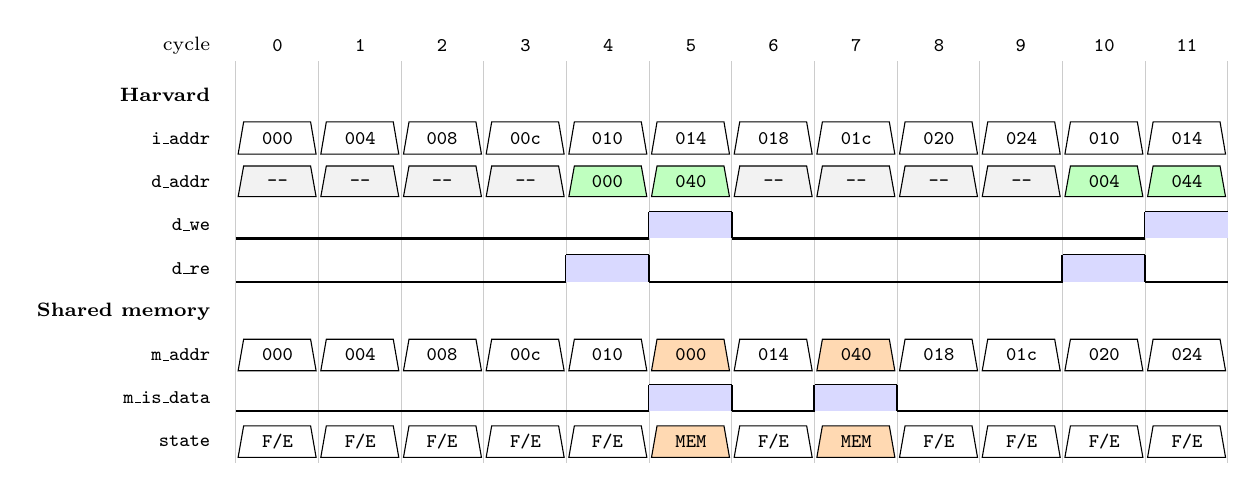
\begin{tikzpicture}[font=\scriptsize\ttfamily, x=1cm, y=1cm]
\node at (0.53,0.35) {0};
\node at (1.58,0.35) {1};
\node at (2.62,0.35) {2};
\node at (3.68,0.35) {3};
\node at (4.73,0.35) {4};
\node at (5.78,0.35) {5};
\node at (6.83,0.35) {6};
\node at (7.88,0.35) {7};
\node at (8.93,0.35) {8};
\node at (9.97,0.35) {9};
\node at (11.03,0.35) {10};
\node at (12.08,0.35) {11};
\node[anchor=east] at (-0.2,0.35) {\normalfont cycle};
\draw[gray!40] (0.00,0.15) -- (0.00,-4.95);
\draw[gray!40] (1.05,0.15) -- (1.05,-4.95);
\draw[gray!40] (2.10,0.15) -- (2.10,-4.95);
\draw[gray!40] (3.15,0.15) -- (3.15,-4.95);
\draw[gray!40] (4.20,0.15) -- (4.20,-4.95);
\draw[gray!40] (5.25,0.15) -- (5.25,-4.95);
\draw[gray!40] (6.30,0.15) -- (6.30,-4.95);
\draw[gray!40] (7.35,0.15) -- (7.35,-4.95);
\draw[gray!40] (8.40,0.15) -- (8.40,-4.95);
\draw[gray!40] (9.45,0.15) -- (9.45,-4.95);
\draw[gray!40] (10.50,0.15) -- (10.50,-4.95);
\draw[gray!40] (11.55,0.15) -- (11.55,-4.95);
\draw[gray!40] (12.60,0.15) -- (12.60,-4.95);
\node[anchor=east,font=\normalfont\bfseries\scriptsize] at (-0.2,-0.28) {Harvard};
\node[anchor=east] at (-0.2,-0.83) {i\_addr};
\draw[fill=white] (0.03,-1.03) -- (0.10,-0.62) -- (0.95,-0.62) -- (1.02,-1.03) -- cycle;
\node at (0.53,-0.83) {000};
\draw[fill=white] (1.08,-1.03) -- (1.15,-0.62) -- (2.00,-0.62) -- (2.07,-1.03) -- cycle;
\node at (1.58,-0.83) {004};
\draw[fill=white] (2.13,-1.03) -- (2.20,-0.62) -- (3.05,-0.62) -- (3.12,-1.03) -- cycle;
\node at (2.62,-0.83) {008};
\draw[fill=white] (3.18,-1.03) -- (3.25,-0.62) -- (4.10,-0.62) -- (4.17,-1.03) -- cycle;
\node at (3.68,-0.83) {00c};
\draw[fill=white] (4.23,-1.03) -- (4.30,-0.62) -- (5.15,-0.62) -- (5.22,-1.03) -- cycle;
\node at (4.72,-0.83) {010};
\draw[fill=white] (5.28,-1.03) -- (5.35,-0.62) -- (6.20,-0.62) -- (6.27,-1.03) -- cycle;
\node at (5.78,-0.83) {014};
\draw[fill=white] (6.33,-1.03) -- (6.40,-0.62) -- (7.25,-0.62) -- (7.32,-1.03) -- cycle;
\node at (6.83,-0.83) {018};
\draw[fill=white] (7.38,-1.03) -- (7.45,-0.62) -- (8.30,-0.62) -- (8.37,-1.03) -- cycle;
\node at (7.88,-0.83) {01c};
\draw[fill=white] (8.43,-1.03) -- (8.50,-0.62) -- (9.35,-0.62) -- (9.42,-1.03) -- cycle;
\node at (8.93,-0.83) {020};
\draw[fill=white] (9.48,-1.03) -- (9.55,-0.62) -- (10.40,-0.62) -- (10.47,-1.03) -- cycle;
\node at (9.98,-0.83) {024};
\draw[fill=white] (10.53,-1.03) -- (10.60,-0.62) -- (11.45,-0.62) -- (11.52,-1.03) -- cycle;
\node at (11.03,-0.83) {010};
\draw[fill=white] (11.58,-1.03) -- (11.65,-0.62) -- (12.50,-0.62) -- (12.57,-1.03) -- cycle;
\node at (12.08,-0.83) {014};
\node[anchor=east] at (-0.2,-1.38) {d\_addr};
\draw[fill=gray!10] (0.03,-1.57) -- (0.10,-1.18) -- (0.95,-1.18) -- (1.02,-1.57) -- cycle;
\node at (0.53,-1.38) {--};
\draw[fill=gray!10] (1.08,-1.57) -- (1.15,-1.18) -- (2.00,-1.18) -- (2.07,-1.57) -- cycle;
\node at (1.58,-1.38) {--};
\draw[fill=gray!10] (2.13,-1.57) -- (2.20,-1.18) -- (3.05,-1.18) -- (3.12,-1.57) -- cycle;
\node at (2.62,-1.38) {--};
\draw[fill=gray!10] (3.18,-1.57) -- (3.25,-1.18) -- (4.10,-1.18) -- (4.17,-1.57) -- cycle;
\node at (3.68,-1.38) {--};
\draw[fill=green!25] (4.23,-1.57) -- (4.30,-1.18) -- (5.15,-1.18) -- (5.22,-1.57) -- cycle;
\node at (4.72,-1.38) {000};
\draw[fill=green!25] (5.28,-1.57) -- (5.35,-1.18) -- (6.20,-1.18) -- (6.27,-1.57) -- cycle;
\node at (5.78,-1.38) {040};
\draw[fill=gray!10] (6.33,-1.57) -- (6.40,-1.18) -- (7.25,-1.18) -- (7.32,-1.57) -- cycle;
\node at (6.83,-1.38) {--};
\draw[fill=gray!10] (7.38,-1.57) -- (7.45,-1.18) -- (8.30,-1.18) -- (8.37,-1.57) -- cycle;
\node at (7.88,-1.38) {--};
\draw[fill=gray!10] (8.43,-1.57) -- (8.50,-1.18) -- (9.35,-1.18) -- (9.42,-1.57) -- cycle;
\node at (8.93,-1.38) {--};
\draw[fill=gray!10] (9.48,-1.57) -- (9.55,-1.18) -- (10.40,-1.18) -- (10.47,-1.57) -- cycle;
\node at (9.98,-1.38) {--};
\draw[fill=green!25] (10.53,-1.57) -- (10.60,-1.18) -- (11.45,-1.18) -- (11.52,-1.57) -- cycle;
\node at (11.03,-1.38) {004};
\draw[fill=green!25] (11.58,-1.57) -- (11.65,-1.18) -- (12.50,-1.18) -- (12.57,-1.57) -- cycle;
\node at (12.08,-1.38) {044};
\node[anchor=east] at (-0.2,-1.93) {d\_we};
\draw[thick] (0.00,-2.10) -- (1.05,-2.10);
\draw[thick] (1.05,-2.10) -- (2.10,-2.10);
\draw[thick] (2.10,-2.10) -- (3.15,-2.10);
\draw[thick] (3.15,-2.10) -- (4.20,-2.10);
\draw[thick] (4.20,-2.10) -- (5.25,-2.10);
\draw[thick] (5.25,-1.76) -- (6.30,-1.76);
\draw[thick] (5.25,-2.10) -- (5.25,-1.76);
\fill[blue!15] (5.25,-2.10) rectangle (6.30,-1.76);
\draw[thick] (6.30,-2.10) -- (7.35,-2.10);
\draw[thick] (6.30,-2.10) -- (6.30,-1.76);
\draw[thick] (7.35,-2.10) -- (8.40,-2.10);
\draw[thick] (8.40,-2.10) -- (9.45,-2.10);
\draw[thick] (9.45,-2.10) -- (10.50,-2.10);
\draw[thick] (10.50,-2.10) -- (11.55,-2.10);
\draw[thick] (11.55,-1.76) -- (12.60,-1.76);
\draw[thick] (11.55,-2.10) -- (11.55,-1.76);
\fill[blue!15] (11.55,-2.10) rectangle (12.60,-1.76);
\node[anchor=east] at (-0.2,-2.48) {d\_re};
\draw[thick] (0.00,-2.65) -- (1.05,-2.65);
\draw[thick] (1.05,-2.65) -- (2.10,-2.65);
\draw[thick] (2.10,-2.65) -- (3.15,-2.65);
\draw[thick] (3.15,-2.65) -- (4.20,-2.65);
\draw[thick] (4.20,-2.31) -- (5.25,-2.31);
\draw[thick] (4.20,-2.65) -- (4.20,-2.31);
\fill[blue!15] (4.20,-2.65) rectangle (5.25,-2.31);
\draw[thick] (5.25,-2.65) -- (6.30,-2.65);
\draw[thick] (5.25,-2.65) -- (5.25,-2.31);
\draw[thick] (6.30,-2.65) -- (7.35,-2.65);
\draw[thick] (7.35,-2.65) -- (8.40,-2.65);
\draw[thick] (8.40,-2.65) -- (9.45,-2.65);
\draw[thick] (9.45,-2.65) -- (10.50,-2.65);
\draw[thick] (10.50,-2.31) -- (11.55,-2.31);
\draw[thick] (10.50,-2.65) -- (10.50,-2.31);
\fill[blue!15] (10.50,-2.65) rectangle (11.55,-2.31);
\draw[thick] (11.55,-2.65) -- (12.60,-2.65);
\draw[thick] (11.55,-2.65) -- (11.55,-2.31);
\node[anchor=east,font=\normalfont\bfseries\scriptsize] at (-0.2,-3.03) {Shared memory};
\node[anchor=east] at (-0.2,-3.58) {m\_addr};
\draw[fill=white] (0.03,-3.78) -- (0.10,-3.38) -- (0.95,-3.38) -- (1.02,-3.78) -- cycle;
\node at (0.53,-3.58) {000};
\draw[fill=white] (1.08,-3.78) -- (1.15,-3.38) -- (2.00,-3.38) -- (2.07,-3.78) -- cycle;
\node at (1.58,-3.58) {004};
\draw[fill=white] (2.13,-3.78) -- (2.20,-3.38) -- (3.05,-3.38) -- (3.12,-3.78) -- cycle;
\node at (2.62,-3.58) {008};
\draw[fill=white] (3.18,-3.78) -- (3.25,-3.38) -- (4.10,-3.38) -- (4.17,-3.78) -- cycle;
\node at (3.68,-3.58) {00c};
\draw[fill=white] (4.23,-3.78) -- (4.30,-3.38) -- (5.15,-3.38) -- (5.22,-3.78) -- cycle;
\node at (4.72,-3.58) {010};
\draw[fill=orange!30] (5.28,-3.78) -- (5.35,-3.38) -- (6.20,-3.38) -- (6.27,-3.78) -- cycle;
\node at (5.78,-3.58) {000};
\draw[fill=white] (6.33,-3.78) -- (6.40,-3.38) -- (7.25,-3.38) -- (7.32,-3.78) -- cycle;
\node at (6.83,-3.58) {014};
\draw[fill=orange!30] (7.38,-3.78) -- (7.45,-3.38) -- (8.30,-3.38) -- (8.37,-3.78) -- cycle;
\node at (7.88,-3.58) {040};
\draw[fill=white] (8.43,-3.78) -- (8.50,-3.38) -- (9.35,-3.38) -- (9.42,-3.78) -- cycle;
\node at (8.93,-3.58) {018};
\draw[fill=white] (9.48,-3.78) -- (9.55,-3.38) -- (10.40,-3.38) -- (10.47,-3.78) -- cycle;
\node at (9.98,-3.58) {01c};
\draw[fill=white] (10.53,-3.78) -- (10.60,-3.38) -- (11.45,-3.38) -- (11.52,-3.78) -- cycle;
\node at (11.03,-3.58) {020};
\draw[fill=white] (11.58,-3.78) -- (11.65,-3.38) -- (12.50,-3.38) -- (12.57,-3.78) -- cycle;
\node at (12.08,-3.58) {024};
\node[anchor=east] at (-0.2,-4.12) {m\_is\_data};
\draw[thick] (0.00,-4.29) -- (1.05,-4.29);
\draw[thick] (1.05,-4.29) -- (2.10,-4.29);
\draw[thick] (2.10,-4.29) -- (3.15,-4.29);
\draw[thick] (3.15,-4.29) -- (4.20,-4.29);
\draw[thick] (4.20,-4.29) -- (5.25,-4.29);
\draw[thick] (5.25,-3.96) -- (6.30,-3.96);
\draw[thick] (5.25,-4.29) -- (5.25,-3.96);
\fill[blue!15] (5.25,-4.29) rectangle (6.30,-3.96);
\draw[thick] (6.30,-4.29) -- (7.35,-4.29);
\draw[thick] (6.30,-4.29) -- (6.30,-3.96);
\draw[thick] (7.35,-3.96) -- (8.40,-3.96);
\draw[thick] (7.35,-4.29) -- (7.35,-3.96);
\fill[blue!15] (7.35,-4.29) rectangle (8.40,-3.96);
\draw[thick] (8.40,-4.29) -- (9.45,-4.29);
\draw[thick] (8.40,-4.29) -- (8.40,-3.96);
\draw[thick] (9.45,-4.29) -- (10.50,-4.29);
\draw[thick] (10.50,-4.29) -- (11.55,-4.29);
\draw[thick] (11.55,-4.29) -- (12.60,-4.29);
\node[anchor=east] at (-0.2,-4.68) {state};
\draw[fill=white] (0.03,-4.88) -- (0.10,-4.48) -- (0.95,-4.48) -- (1.02,-4.88) -- cycle;
\node at (0.53,-4.68) {F/E};
\draw[fill=white] (1.08,-4.88) -- (1.15,-4.48) -- (2.00,-4.48) -- (2.07,-4.88) -- cycle;
\node at (1.58,-4.68) {F/E};
\draw[fill=white] (2.13,-4.88) -- (2.20,-4.48) -- (3.05,-4.48) -- (3.12,-4.88) -- cycle;
\node at (2.62,-4.68) {F/E};
\draw[fill=white] (3.18,-4.88) -- (3.25,-4.48) -- (4.10,-4.48) -- (4.17,-4.88) -- cycle;
\node at (3.68,-4.68) {F/E};
\draw[fill=white] (4.23,-4.88) -- (4.30,-4.48) -- (5.15,-4.48) -- (5.22,-4.88) -- cycle;
\node at (4.72,-4.68) {F/E};
\draw[fill=orange!30] (5.28,-4.88) -- (5.35,-4.48) -- (6.20,-4.48) -- (6.27,-4.88) -- cycle;
\node at (5.78,-4.68) {MEM};
\draw[fill=white] (6.33,-4.88) -- (6.40,-4.48) -- (7.25,-4.48) -- (7.32,-4.88) -- cycle;
\node at (6.83,-4.68) {F/E};
\draw[fill=orange!30] (7.38,-4.88) -- (7.45,-4.48) -- (8.30,-4.48) -- (8.37,-4.88) -- cycle;
\node at (7.88,-4.68) {MEM};
\draw[fill=white] (8.43,-4.88) -- (8.50,-4.48) -- (9.35,-4.48) -- (9.42,-4.88) -- cycle;
\node at (8.93,-4.68) {F/E};
\draw[fill=white] (9.48,-4.88) -- (9.55,-4.48) -- (10.40,-4.48) -- (10.47,-4.88) -- cycle;
\node at (9.98,-4.68) {F/E};
\draw[fill=white] (10.53,-4.88) -- (10.60,-4.48) -- (11.45,-4.48) -- (11.52,-4.88) -- cycle;
\node at (11.03,-4.68) {F/E};
\draw[fill=white] (11.58,-4.88) -- (11.65,-4.48) -- (12.50,-4.48) -- (12.57,-4.88) -- cycle;
\node at (12.08,-4.68) {F/E};
\end{tikzpicture}
}
  \caption{Phase I, first twelve cycles of \sig{memcopy}, generated from the simulation trace by
  \sig{tools/vcd2tikz.py}. On the Harvard system the data address is active in the same cycle as
  the instruction address. On the baseline every LW/SW occupies an extra \textsc{Mem} cycle on
  the shared bus.}
  \label{fig:wave1}
\end{figure*}

In Phase~I, Yosys synthesis for a Xilinx 7-series target gave 654 LUTs for the Harvard system
(including a separately synthesised ROM) and 1084 for the baseline, and place-and-route on a
Lattice ECP5 gave 43.6\,MHz and 37.4\,MHz. The Phase~I report and its scripts are kept unchanged
in the repository (\sig{report/phase1/}, \sig{results/synth/}, \sig{results/fmax/}).
